%% SOURCE: experiments/010-kuzmin-tmi/scripts/strong_positive_candidates.py -- counts from results/strong_positive_counts.csv, triples from results/strong_positive_triples.csv, cost from results/strong_positive_summary.json; retrieval rows from positive_interaction_retrieval.py

\section{Restricting to strong interactions\secstatus{todo}}

Requiring the model to call an interaction \emph{strong} rather than merely
positive shrinks the pool by two orders of magnitude and removes the diversity
the panel was built around.

\subsection{Where the threshold comes from\secstatus{todo}}

Kuzmin's ordinary call is a conjunction at $|{\cdot}| > 0.08$ with $p < 0.05$.
Baryshnikova 2010 adds a stringent tier that is sign-asymmetric,
$\varepsilon < -0.12$ negative and $\varepsilon > 0.16$ positive, and the
positive arm is the strong cut used here. It is a digenic threshold applied to a
trigenic score, which is an approximation rather than a published standard: no
stringent tier for positive \emph{trigenic} interactions exists.

\subsection{How many\secstatus{todo}}

\begin{table}[H]
\centering
\begin{tabular}{lrrr}
\toprule
Predicted $\tau$ cut & by ensemble mean & every checkpoint above & distinct genes \\
\midrule
$> +0.08$ & 209 & 39 & 23 \\
$> +0.12$ & 74  & 24 & 14 \\
$> +0.16$ \emph{(strong)} & \textbf{39} & \textbf{15} & \textbf{10} \\
$> +0.20$ & 29  & 13 & 8 \\
$> +0.30$ & 18  & 11 & 7 \\
$> +0.50$ & 8   & 7  & 6 \\
\bottomrule
\end{tabular}
\caption{Triples of the 4{,}370{,}595 in \texttt{inference\_1} clearing each cut.
The two columns differ by $2.6$ times at the strong cut because a mean can be
carried by one optimistic checkpoint. Requiring all three is the rule a build
list should use.}
\end{table}

So the answer is \textbf{15 triples}, over 10 genes, under the conservative rule.
Two fail the training-support gate, \texttt{YGR193C} at 10 records and
\texttt{YHL003C} at 0, which leaves \textbf{13 triples over 8 genes}.

\subsection{What it costs and what it removes\secstatus{todo}}

\begin{table}[H]
\centering
\begin{tabular}{lrr}
\toprule
& strong only & two-block design \\
\midrule
triples                     & 13 & 20 \\
genes                       & 8  & 10 \\
doubles for $\tau$ closure  & 19 & 20 \\
strains on the plate        & 41 & 51 \\
triples containing \texttt{YER059W} & 12 of 13 & 6 of 20 \\
control arm                 & none & 10 triples \\
\bottomrule
\end{tabular}
\caption{The strong restriction is 10 strains cheaper and loses both the
generalization control and the balance.}
\end{table}

The concentration becomes total. Twelve of the 13 gated strong triples contain
\texttt{YER059W}, and the single exception is
\texttt{YBR001C + YHR003C + YPL181W} at $+0.481$. Every gene participation count
is set by that one gene: no complete block survives the cut, so the design
reverts to a ranked list.

\subsection{The tier is retrievable, at low absolute precision\secstatus{todo}}

\begin{table}[H]
\centering
\begin{tabular}{lrrr}
\toprule
Model & P@100 & enrichment & average precision \\
\midrule
\multicolumn{4}{l}{\emph{$\tau > +0.16$ and $p < 0.05$, base rate 0.181\%}} \\
B1 additive ridge & 0.030 & 16.6$\times$ & 0.0069 \\
B5 nonlinear MLP  & 0.020 & 11.1$\times$ & 0.0081 \\
CGT ensemble      & 0.070 & 38.8$\times$ & 0.0300 \\
\bottomrule
\end{tabular}
\caption{Retrieval at the strong tier on the random-over-records test split. The
transformer's average precision is $4.3$ times the additive null's, wider than
the $3.2$ at the ordinary call, but only 7 of its 100 most positive predictions
are real strong calls.}
\end{table}

The margin over the additive null widens as the tier tightens, $1.9$ times at the
negative call, $3.2$ at the ordinary positive call, $4.3$ here and $7.2$ at
$\tau > +0.20$. Absolute precision falls the other way, so a strong-only list is
a higher-confidence ranking of a much rarer event, not a more reliable one.

On the query-pair-disjoint split the strong tier holds 13 positives in 37{,}680
records and both baselines retrieve none of them in their top 1{,}000. That
comparison is not evidence of collapse, it is an absence of measurable signal at
this rarity, and the transformer is unmeasured there either way.

\begin{figure}[H]
\centering
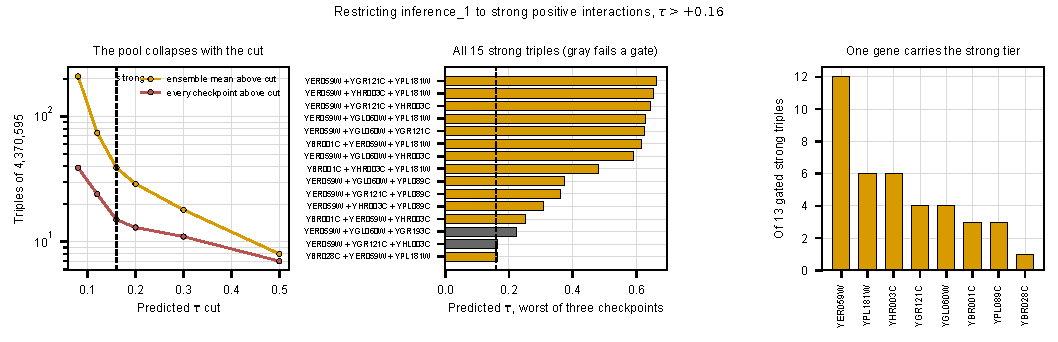
\includegraphics[width=\linewidth]{figures/strong_positive_candidates.pdf}
\caption{The strong pool. Gray bars fail a gene gate. Generated by
\protect\file{experiments/010-kuzmin-tmi/scripts/strong_positive_candidates.py}.}
\end{figure}

\subsection{The choice this forces\secstatus{todo}}

Building only strong predictions buys a higher bar on 13 triples and gives up the
contrast that made the 20-triple design readable. If tier A of that design
measures high, the strong-only list would have measured high too, and neither
would say whether the model ranks interactions or one gene. Keeping four
non-\texttt{YER059W} triples from the same block and ten from a disjoint block
costs 10 strains and is what separates those two outcomes.
